%% =====================================================================
%%  contenido.tex — Cuerpo del artículo. VERSIÓN CORTA (equivalente a la
%%  entrega de 12 páginas: la tabla de responsabilidades por capa y el
%%  banco de pruebas quedan en el material suplementario).
%% =====================================================================

\section{Introducción}\label{sec:intro}
Kubernetes es hoy la plataforma de facto para orquestar cargas en contenedores, incluidas las bases de datos \citep{schwarzkopf2013,burns2016}, lo que ha favorecido el desarrollo de operadores —en particular para PostgreSQL— que automatizan el ciclo de vida, la replicación y el \textit{failover} \citep{dobies2020,k8s2026operator}. En paralelo, la \textit{Container Storage Interface} (CSI) estandariza la integración de almacenamiento heterogéneo \citep{k8s2024csi}. La literatura tiende a analizar estos componentes por separado \citep{gilbert2002,bailis2013}, pese a que la recuperación ante fallos depende de su interacción \citep{avizienis2004}.

Este artículo mide el coste del \textit{failover} de CloudNativePG en un clúster productivo y examina, para cada fallo inyectado, si el inyector reprodujo el fallo que nombra. Presenta:
\begin{itemize}[leftmargin=1.2em,itemsep=2pt,topsep=2pt]
\item Una taxonomía de operadores y de almacenamiento CSI, con un vocabulario común —el modelo $S=(O,K,M,D)$ y sus invariantes—, sin pretensión predictiva.
\item La medición del coste del \textit{failover} de CloudNativePG ante la eliminación del primario: RTO mediano de 7,9~s y RPO nulo en diez repeticiones.
\item El hallazgo metodológico central: de los cuatro escenarios diseñados, solo uno produjo el fallo que nominalmente modela. El \textit{pod-failure} de Chaos Mesh altera la especificación del pod, lo que —se argumenta— plantea una deriva y no una indisponibilidad; la \textit{NetworkPolicy} no aisló al primario del plano de control; y el inyector de E/S es incompatible con el endurecimiento del operador. Validar el inyector es, en operadores declarativos, condición previa a cualquier cifra de resiliencia.
\end{itemize}
Es un estudio piloto, acotado por las restricciones del clúster productivo (\refsec{sec:metodo}).

\section{Trabajos relacionados}\label{sec:rel}
Tres líneas convergen aquí. La \emph{orquestación de clústeres} arranca en Borg y Omega \citep{schwarzkopf2013,burns2016}, donde la CSI abstrae el almacenamiento persistente \citep{k8s2024csi} y el patrón \textit{Operator} consolida la gestión declarativa \citep{k8s2026operator}. En \emph{bases de datos distribuidas}, el teorema CAP y sus relecturas \citep{gilbert2002,abadi2012,bailis2013}, con la disponibilidad y la consistencia nombradas según la taxonomía canónica de la \textit{dependability} \citep{avizienis2004}. Y la \emph{recuperación y replicación}, que aporta el WAL \citep{mohan1992,han2024}. El despliegue \textit{stateful} mediante operadores ha ganado atención \citep{dobies2020,mega2023}, pero rara vez caracteriza el comportamiento ante fallos inyectados.

Una cuarta vertiente, metodológica, verifica la resiliencia por inyección controlada: el \textit{chaos engineering} \citep{basiri2016}, la inyección dirigida por linaje \citep{alvaro2018} y la caracterización de particiones en producción \citep{alquraan2018}. Para consistencia y durabilidad, la referencia canónica es Jepsen con su verificador Elle \citep{kingsbury2020}; el \textit{tx-verifier} comparte ese espíritu con alcance más acotado: durabilidad a nivel de \textit{commit} sobre un operador concreto. El propio CloudNativePG integra pruebas de caos en su integración continua, con comprobaciones de estilo Jepsen y métricas de \textit{failover} \citep{drees2026}, orientadas a la no regresión del proyecto y no al coste del fallo en un despliegue dado; \citet{chen2026} evalúan el plano de orquestación, no un operador con estado. La fiabilidad de los operadores en sí se ataca con pruebas automáticas —Sieve \citep{sun2022} y Acto \citep{gu2023}—, que recorren el espacio de estados del controlador: su objeto es el operador como programa, no el coste observable del fallo. En sentido inverso, trabajo independiente reprodujo un \textit{split-brain} en CloudNativePG bajo aislamiento completo, con escrituras confirmadas y luego perdidas \citep{sivko2026}, resultado que acota la lectura de los escenarios de partición (\refsec{sec:res}). La brecha que se cierra no es la ausencia de inyección de fallos en Kubernetes, sino la de una medición a nivel de \textit{commit} sobre un operador de PostgreSQL en producción, acompañada del examen de si el inyector produjo el fallo que nombra.

\section{Marco de análisis}\label{sec:marco}
\subsection{Taxonomía y modelo del sistema}\label{sec:taxo}
Los operadores de PostgreSQL se ordenan aquí por \emph{quién decide la promoción}, que es la dimensión pertinente ante un fallo: en CloudNativePG (CNPG) decide el operador, dentro del bucle de reconciliación; en Zalando Postgres Operator y en Crunchy Postgres for Kubernetes~v5 decide Patroni en cada pod, por elección de líder sobre una clave con tiempo de vida. Ni la fuente de verdad ni el modelo de almacenamiento los separan: ambos enfoques descansan en el \textit{API server} y siguen una arquitectura \textit{shared-nothing} (\refsec{sec:reparto}). De la decisión central cabe esperar mayor coherencia con el ciclo de vida de Kubernetes, y de la distribuida un perfil distinto de latencia de detección; son expectativas documentadas, no medidas aquí \citep{dobies2020,k8s2026operator}. El estudio se limita a CNPG por una restricción del entorno (\refsec{sec:metodo}); el contraste con los demás es analítico (Tabla~S2 del suplemento).

El almacenamiento se ordena por \emph{dónde reside el dominio de fallo del volumen} \citep{k8s2024csi}: \textit{adosado al nodo} (disco local, muere con él); \textit{replicado}, cuando el propio sistema mantiene copias en varios nodos (Ceph, Longhorn); y \textit{externo al clúster} (SAN, NFS), que sobrevive a la caída de cualquier nodo a costa de depender de la conectividad. El criterio hace las categorías excluyentes, cosa que las etiquetas habituales no logran: Ceph RBD y una SAN se acceden ambos por red, pero su dominio de fallo difiere. El piloto usa almacenamiento externo al clúster.

Sobre esa taxonomía, el sistema se describe como una tupla, según la \refec{eq:modelo}:
\begin{equation}\label{eq:modelo}
S = (O, K, M, D)
\end{equation}
Donde $O$ es la lógica del operador, $K$ el plano de control de Kubernetes, $M$ la capa de almacenamiento gestionada mediante CSI y $D$ el motor de base de datos \citep{schwarzkopf2013,burns2016,k8s2024csi}. No es una formulación matemática sino un vocabulario descriptivo, andamiaje para razonar sobre cómo las decisiones de una capa se propagan al comportamiento global bajo fallo. Sobre él se organizan tres dimensiones de observación, enunciadas como tales  (qué se mira y con qué variable) y no como relaciones formales, porque a este nivel de evidencia una ecuación no añadiría contenido verificable: la \textit{resiliencia}, mediante el tipo de fallo, el tiempo de restablecimiento y la disponibilidad posterior \citep{avizienis2004}; la \textit{consistencia}, mediante la diferencia entre transacciones confirmadas al cliente y transacciones visibles tras el fallo —donde la relectura PACELC es pertinente, pues el compromiso no se da solo entre consistencia y disponibilidad bajo partición, sino también entre consistencia y latencia en operación normal \citep{gilbert2002,abadi2012,bailis2013}—; y la \textit{interacción multicapa}, mediante el reparto de responsabilidades que instancia la Tabla~S2 del material suplementario.

\subsection{Invariantes del sistema}\label{sec:inv}
Tres invariantes delimitan un comportamiento aceptable bajo fallo. El de \textit{consistencia}: toda transacción confirmada debe permanecer accesible tras la recuperación \citep{bailis2013}. El de \textit{durabilidad}: toda operación registrada en el \textit{log} de escritura anticipada debe ser recuperable, según el protocolo canónico y su linaje posterior \citep{mohan1992,han2024}. El tiempo de recuperación (RTO) se trata, en cambio, como métrica observable y no como invariante: sin un objetivo de nivel de servicio declarado a priori, se mide y se contrasta entre escenarios, y es cada despliegue el que puede elevarlo a umbral de conformidad \citep{avizienis2004}. Los tres se operacionalizan en las Secciones~\ref{sec:metodo} y~\ref{sec:res} mediante RPO, latencia de \textit{failover} y pérdida de transacciones.

\subsection{Reparto de responsabilidades por capa}\label{sec:reparto}
El comportamiento del sistema no se explica capa por capa de forma aislada. El material suplementario recoge, en su Tabla~S2, el reparto de responsabilidades de detección y recuperación entre capas para los tipos de fallo pertinentes, a partir del comportamiento documentado de CloudNativePG \citep{cnpg2026}, Zalando Postgres Operator mediante Patroni \citep{patroni2026} y Crunchy Postgres for Kubernetes \citep{crunchy2026}; es una síntesis analítica y no una medición. Tres de sus entradas conviene traerlas aquí, porque corrigen lecturas habituales.



Ante el fallo del pod primario, $O$ detecta y promueve, $K$ restablece el enrutamiento y $D$ retoma escrituras: el RTO emerge de la composición temporal de esas acciones. Importa quién hace qué, porque CNPG gestiona los pods directamente, sin \textit{StatefulSet}: no es el \textit{kubelet} quien recrea el pod, sino el propio operador. Ante el fallo del nodo, la secuencia es más larga de lo que suele suponerse: el plano de control marca el nodo \textit{NotReady} tras $\approx$50~s  (valor por defecto de \texttt{node-monitor-grace-period} en Kubernetes~v1.34; la documentación de CNPG lo sitúa entre 40 y 55~s), y el desalojo por marca no llega hasta agotarse la tolerancia, de 300~s por defecto \citep{k8s2026kcm}. No hay que confundir desalojo con desaparición: en un nodo inalcanzable el \textit{kubelet} no puede confirmar la terminación, así que el objeto Pod permanece en \textit{Terminating} hasta que se borre el objeto Node o se aplique la marca \texttt{node.kubernetes.io/\allowbreak out-of-\allowbreak service}. El primario no pierde, por tanto, su identidad en el registro; CNPG promueve porque detecta la instancia como no sana, no porque el pod deje de existir. Ante una partición, el cercado (\textit{fencing}) expone un contraste que suele enunciarse mal: en Kubernetes, Patroni no despliega un etcd propio, sino que emplea objetos nativos del clúster  (\textit{Endpoints} o \textit{ConfigMaps}) como DCS, igual que Zalando Postgres Operator (Spilo) y Crunchy PGO~v5. Los tres descansan, pues, en el \textit{API server}; lo que los separa es quién decide la promoción.


\section{Metodología experimental}\label{sec:metodo}
Todo lo que se afirma en esta sección y en la siguiente es auditable: los manifiestos del clúster, de la carga y de cada inyección, el \textit{tx-verifier}, los scripts de análisis y las series de RTO y RPO por repetición están depositados en Zenodo (DOI: 10.5281/\allowbreak zenodo.23004248), y se citan en adelante por su ruta dentro del paquete.

\subsection{Entorno, aislamiento y alcance}\label{sec:entorno}
El experimento se ejecutó sobre un clúster Kubernetes en producción (v1.34.6) con PostgreSQL 16.13, CloudNativePG (CNPG) 1.28.0, red gestionada por Calico 3.31.4 y almacenamiento en red del controlador CSI de Huawei 4.10.1 (\texttt{csi.huawei.com}) sobre \textit{Fibre Channel}, aprovisionado por una \textit{StorageClass} con retención de volúmenes y enlace diferido al primer consumidor.

La ejecución se acordó con el equipo de operaciones del clúster, que autorizó el experimento acotado a un espacio de nombres dedicado y no permitió instalar operadores nuevos por el riesgo sobre las cargas en producción; de ahí que el alcance se limite a CNPG, y que el contraste con los enfoques basados en Patroni se aborde de forma analítica (Tabla~S2) y se asigne a la Fase~2. Esa decisión deja dos fuentes de varianza fuera de control que conviene declarar. La primera: el operador CNPG era el mismo que atendía otros cuatro clústeres del entorno, luego su carga de reconciliación —no instrumentada— pudo afectar a la latencia de detección. La segunda: el nodo del laboratorio alojaba además instancias primarias ajenas al experimento, y ni la CPU ni la E/S del nodo se registraron durante las rondas.

La inyección se realizó con Chaos Mesh 2.8.3 en un entorno \textit{air-gapped}, dentro de un espacio de nombres dedicado con cuotas y control de acceso, por lo que las cargas productivas quedaron fuera del dominio de fallo. El aislamiento descansó en tres controles —Chaos Mesh restringido al espacio de nombres, doble filtro de selección en cada manifiesto y verificación previa (\textit{dry-run}) de cada selector— y en excluir los pods de la malla de servicios para no sesgar las mediciones (detalle en el material suplementario).

El manifiesto declaraba antiafinidad entre instancias en su modalidad \emph{preferente}, que es la que CNPG aplica por defecto; como el \textit{pool} de nodos elegibles se reducía a uno, el planificador la incumplió sin bloquear el despliegue y las tres instancias residieron en el mismo nodo (Fig.~S1 del suplemento). El \textit{failover} observado fue intranodo y el fallo de nodo completo no era comprobable por construcción (\refsec{sec:disc}).


\subsection{Carga de trabajo y cliente de verificación}\label{sec:carga}
El operador desplegó un clúster de tres instancias sometido a una carga sintética continua generada con pgbench (escala \texttt{-s 10}, 4 clientes y 2 hilos concurrentes), en rondas sucesivas de 60~s que toleraban \textit{failovers}. La replicación entre instancias se mantuvo en su modo asíncrono por defecto \citep{postgresql2024}; el modo síncrono no se varió en este piloto, de modo que las cifras de RPO reportadas corresponden a replicación asíncrona.

En paralelo, un cliente de verificación (\textit{tx-verifier}) insertó identificadores BIGINT monótonos y anotó cada COMMIT con su marca de tiempo; ante un fallo reintentó el mismo identificador, y por eso un hueco en la tabla de verdad equivale a una escritura reconocida y perdida (\textit{proxy} del RPO). El alcance del reintento es más estrecho de lo que parece: el cliente redirige el error a \texttt{/dev/null}, así que una violación de clave duplicada (la firma de un \textit{commit} que sí persistió) es indistinguible de un fallo de conexión. El diseño no detecta, pues, el \textit{commit} fantasma; de darse, habría reintentado el mismo identificador sin fin, y no se observó tal cosa. El comportamiento del cliente forma parte de la medición, así que conviene detallarlo (\texttt{30-workload/\allowbreak tx-verifier-cnpg.yaml}): cada inserción es una invocación independiente de \texttt{psql} sobre libpq contra el servicio \texttt{-rw} del clúster, por lo que abre una conexión nueva en cada iteración y no media ningún \textit{pooler}; el tiempo de espera de conexión se fijó en 2~s (\texttt{PGCONNECT\_TIMEOUT}) y el resto de parámetros de libpq, incluido el \textit{keepalive} de TCP, quedaron en sus valores por defecto; ante un fallo el cliente espera 0,2~s y reintenta el mismo identificador. El RTO reportado engloba, por tanto, la detección por el operador, la promoción, la actualización de los \textit{Endpoints} del servicio y el restablecimiento de la conexión del cliente, con una granularidad de $\approx 0{,}2$~s. Descomponerlo en esos tramos exigiría los eventos del plano de control, que no se conservaron (\refsec{sec:rtorpo}).

Quedan así operacionalizados los invariantes de la \refsec{sec:marco}: el RPO como transacciones confirmadas no visibles tras el fallo, y el RTO como el hueco entre la última escritura reconocida y la primera aceptada. Al medirse con el reloj único del cliente, el RTO no depende de la sincronización entre nodos.

\subsection{Escenarios de fallo y tamaño muestral}\label{sec:escenarios}
Se aplicaron tres escenarios reproducibles con seguridad en producción: F1, eliminación del pod primario (PodChaos, modo \textit{pod-kill}); F2, indisponibilidad del primario (modo \textit{pod-failure}), con ventana nominal de 10~min, menor en la práctica (\refsec{sec:rtorpo}); y F3, partición de red del primario mediante una \textit{NetworkPolicy} de Calico, sin Chaos Mesh, aplicada y revertida con \texttt{kubectl}. Un cuarto escenario, F4 —sensibilidad del RTO a la latencia de E/S (0, 20, 50 y 100~ms) por IOChaos sobre FUSE—, resultó no ejecutable (\refsec{sec:io}) y queda para la Fase~2.

F1 se repitió diez veces ($n=10$); se inyectó sin \texttt{gracePeriod} explícito, con lo cual rigió el valor por defecto (0~s) y la terminación fue abrupta, sin apagado ordenado del motor. F2 se inyectó once veces: la primera se descartó por arranque en frío (véase la \refsec{sec:rtorpo}) y las diez restantes componen la muestra analizada ($n=10$); F3, diez veces fijas de 60~s más dos inyecciones exploratorias (149~s y 300~s) excluidas del RTO, sin promoción en las doce (0/12). El tamaño muestral respondió a las ventanas de mantenimiento del clúster. Con $n=10$ y una resolución de instrumento de $\approx0{,}2$~s, lo que se caracteriza es la tendencia central; la dispersión observada en F1 es del orden del error de medida, de modo que no se interpreta. Por la no normalidad esperada se reportan medianas y cuartiles.

Los fallos de nodo no se reprodujeron: el clúster no permite drenar nodos y las tres instancias residían en uno solo (\refsec{sec:entorno}). Y F2 no los sustituye. CNPG es \emph{shared-nothing}: cada instancia posee su PVC, así que la promoción recae en una réplica que ya tiene montado su volumen, y la reasociación del volumen del antiguo primario no está en el camino crítico del \textit{failover} —solo interviene al reincorporarse como réplica—. Ante un fallo de nodo, el RTO estaría dominado por la detección (40--55~s) más la promoción, no por el almacenamiento. El caso se aborda analíticamente (Tabla~S2).

\section{Resultados}\label{sec:res}
Las mediciones sobre CNPG fueron descriptivas (medianas, IQR, intervalos de confianza de mediana) más un único contraste de dos grupos intra-CNPG (F1 frente a F2); por la no normalidad de RTO y RPO se reportaron medianas e IQR.

\subsection{Tiempo de recuperación (RTO) y pérdida de datos (RPO)}\label{sec:rtorpo}
La \reftab{tab:rto} resume los tres escenarios. El RPO fue nulo en todos, pero solo F1 puso a prueba la durabilidad: al promover una réplica, $\text{RPO}=0$ implica que ninguna escritura reconocida sobrevivió únicamente en el primario caído; sin promoción, en F2 y F3 el RPO nulo es trivial. Que CNPG lo preserve en F1 bajo replicación asíncrona es un resultado y no una garantía de diseño, atribuible a un \textit{lag} de replicación $\approx 0$ bajo la carga ligera  (inferencia, no medida: no se registró el LSN, carencia que la Fase~2 subsana) y acotado por la colocalización intranodo (\refsec{sec:disc}). La tabla de verdad resultó contigua, de 1 a 613\,253 sin huecos, una vez descartado un identificador espurio negativo que se registró fuera de toda ventana de inyección. No conviene sobreleer esa contigüidad. El verificador escribe en serie: en cada instante hay, a lo sumo, una transacción en ejecución, de modo que su poder de detección es limitado; con diez inyecciones válidas y cero pérdidas, la cota superior unilateral al 95\,\% para la probabilidad de pérdida por \textit{failover} es del 25,9\,\%. El dato es compatible con un RPO nulo; no lo acredita con fuerza. Las transacciones de pgbench, además, no se verificaron (derivación en el material suplementario). La variabilidad se concentró, pues, en el RTO.

\begin{table}[htbp]
  \centering
  \caption{RTO y RPO por escenario de fallo (CloudNativePG).}
  \label{tab:rto}
  \footnotesize
  \renewcommand{\arraystretch}{1.1}
  \begin{tabularx}{\linewidth}{@{}c c c >{\raggedright\arraybackslash}X c >{\raggedright\arraybackslash}p{1.7cm}@{}}
  \toprule
  \textbf{Esc.} & \textbf{n} & \textbf{¿Prom.?} & \textbf{Indisp. (mediana)} & \textbf{RPO} & \textbf{Comport. observado} \\
  \midrule
  F1 & 10 & Sí & 7,9 s\textsuperscript{a} & 0 & Failover rápido \\
  F2 & 10 & No & 36,7 s & 0 & Reinicio en sitio, mismo PVC \\
  F3 & 10 & No & = duración partición & 0 & Fallo no detectado \\
  F4 & --- & --- & No ejecutable & --- & Bloqueo (FUSE) \\
  \bottomrule
  \end{tabularx}
  \notatabla{Escenarios: F1 = \textit{pod-kill}; F2 = \textit{pod-failure}; F3 = partición de red por \textit{NetworkPolicy}; F4 = latencia de E/S (IOChaos FUSE). RTO = mediana del hueco entre transacciones confirmadas por el cliente de verificación, con granularidad de instrumento de $\approx 0{,}2$~s, a la que se ajusta la precisión reportada (\refsec{sec:carga}); RPO = transacciones confirmadas no visibles tras el fallo. «¿Prom.?» indica si el operador promovió una réplica. \textsuperscript{a}Solo F1 es un tiempo de recuperación en sentido propio; en F2 y F3 no hubo acción de recuperación y la cifra es la duración de la indisponibilidad. \textbf{Solo F1 reprodujo el fallo que nominalmente modela}: la cifra de F2 es atribuible a una reconciliación inducida por el inyector, y en F3 el fallo no llegó a ser visible para el plano de control. Ninguno de los dos escenarios sostiene, por tanto, conclusión alguna sobre la lógica de promoción (inferencia; \refsec{sec:rtorpo}). Muestras: $n=10$ en F1 y F2; en F3, 10 repeticiones de 60~s más 2 exploratorias excluidas del RTO. Fuente: mediciones del piloto.}
\end{table}

En F1 (\textit{pod-kill}), CNPG ejecutó \textit{failover} en las diez repeticiones con un RTO mediano de \textbf{7,9~s} (Q1--Q3: 7,6--8,0~s; rango 6,6--8,2~s). F2 (\textit{pod-failure}) no promovió en ninguna. Sobre la ventana: el manifiesto declara \texttt{duration:\ 10m}, pero el arnés retira la inyección al agotar su bucle de detección de promoción, a los $\approx$120~s, de modo que la ventana efectiva fue de unos dos minutos y no de diez; la recuperación precede con holgura a esa retirada. El operador recreó el pod primario en su sitio, con el mismo nombre e idéntico PVC, con una indisponibilidad mediana de \textbf{36,7~s} (Q1--Q3: 36,2--37,1~s; rango 35,5--38,3~s). F3 tampoco promovió: el pod aislado permaneció \textit{Ready} y la indisponibilidad resultó indistinguible de la duración inyectada ($\approx$61~s para 60~s de política), con recuperación inmediata al retirarla. No se reporta con mayor precisión a propósito: la rejilla de muestreo efectiva en F3 no es la de 0,2~s que rige en F1 y F2, porque la política descarta el tráfico en vez de rechazarlo y cada intento del cliente agota su espera de conexión (suplemento). La cifra de F3 mide cuánto duró la política, no una recuperación: no hubo ninguna que medir. Los intervalos de confianza de mediana y demás detalles estadísticos están en el material suplementario.

La primera de las once inyecciones de F2 (80,54~s, arranque en frío) se excluyó de la mediana. La exclusión es conservadora y de escaso efecto: la mediana de las diez retenidas es de 36,7~s y la de las once, 36,9~s; incluirla \emph{ampliaría} la brecha F1--F2. Se reportan ambas por tratarse de una decisión posterior a la ejecución. Dentro del lote de F2 se observó una asociación orden--RTO de magnitud moderada a fuerte (Spearman $\rho\approx 0{,}62$), que no alcanza significación con $n=10$ ($\rho$ crítico $\approx 0{,}65$) por falta de potencia, no por ser pequeña. Sugiere una deriva entre repeticiones; con todo, su efecto es un orden de magnitud menor que la separación F1--F2 ($\approx 29$~s), por lo que no compromete el contraste. Sí lo acota, en cambio, un rasgo del diseño que las marcas de tiempo depositadas dejan ver: los dos escenarios se ejecutaron en bloques separados —F1 entre las 13:54 y las 14:21~UTC, F2 entre las 22:22 y las 23:03, con una inyección cada $\approx 2{,}5$~min en F1 y cada $\approx 4{,}5$~min en F2—, y por eso el escenario queda confundido con la hora del día y con la carga de un clúster productivo compartido. Cabe esperar, aunque no se midió  (la carga del nodo no se instrumentó), que el sesgo opere en contra del resultado, pues la franja de mayor actividad corresponde a F1, que es el lote rápido; aun así, la alternancia de escenarios dentro de cada bloque queda pendiente para la Fase~2.

Los dos lotes no se solapan (\reffig{fig:timeline}): Mann--Whitney $U=0$ y diferencia de Hodges--Lehmann de 29,0~s. Con $n=10$ el $p$ exacto es el mínimo alcanzable, de modo que el peso probatorio recae en el tamaño del efecto y en el mecanismo, no en el contraste (detalle en el material suplementario). El mecanismo, sin embargo, no es el que una lectura directa sugiere: determinarlo obliga a examinar qué hace realmente cada inyector.

\textit{Qué mide F2.} El escenario \textit{pod-failure} de Chaos Mesh no detiene el proceso de la base de datos: sustituye la imagen del contenedor por una imagen de pausa y sostiene esa sustitución durante la ventana indicada \citep{chaosmesh2026}. Parchear \texttt{image} en un pod en marcha no altera su política de descarga, fijada al crearlo, luego la imagen de pausa debe descargarse. Sobre un operador declarativo, esa modificación de la especificación del pod es ella misma una desviación respecto del estado deseado, y el clúster del piloto se declaró con \texttt{primaryUpdateStrategy:\ unsupervised} (\texttt{20-cluster/\allowbreak cluster-cnpg.yaml} del paquete depositado), sin fijar \texttt{failoverDelay} ni \texttt{primaryUpdateMethod}, por lo que rigen sus valores por defecto: 0~s y reinicio.

Conviene además señalar que la imagen de pausa no figura entre las precargadas en el entorno \textit{air-gapped} (\texttt{images/image-list.txt}), por lo que lo más probable es que no llegara a descargarse y el contenedor quedara en \texttt{ImagePullBackOff}. La conclusión no depende de cuál de los dos cursos ocurriera: en ambos el proceso de base de datos deja de atender, la especificación del pod queda alterada y el operador la reconcilia reiniciando el pod en su sitio —con el mismo nombre y el mismo PVC, que es lo observado—. Los 36,7~s miden entonces cuánto tarda el operador en deshacer la alteración que introdujo la herramienta, no cuánto tarda en reaccionar ante un primario indisponible; la lectura de que «decide esperar» no se sostiene, y el propio manifiesto lo cierra: al no fijarse \texttt{failoverDelay} rige su valor por defecto de 0~s, de modo que, de haber percibido al primario como indisponible, el operador habría promovido sin demora. Que no promoviera es la evidencia de que no percibió indisponibilidad alguna. El segundo curso explicaría además el arranque en frío de la inyección descartada (80,54~s): el tiempo que el primer intento de descarga tarda en agotarse.

Esta reconstrucción es una \emph{inferencia} a partir de los manifiestos depositados y del comportamiento documentado de ambas herramientas, no una observación: los eventos del plano de control y los registros del operador durante las inyecciones no se conservaron, y el entorno productivo ya no está disponible para volver a capturarlos. Discriminar entre las dos ramas, y confirmar el mecanismo, exige repetir F2 con un inyector que no toque la especificación del pod  (\texttt{SIGKILL} sostenido al proceso \texttt{postgres}, o bloqueo del puerto 5432) registrando los eventos del operador. Queda comprometido para la Fase~2 con el diseño ya especificado. Hasta entonces, la cifra de F2 debe leerse como el coste de una reconciliación forzada y no como un RTO.

\textit{Qué mide F3.} La \textit{NetworkPolicy} denegó todo el tráfico de entrada y salida del pod primario, incluido el dirigido al \textit{API server}. No bastó, por dos razones que separar. La primera estaba anotada en los comentarios del propio manifiesto depositado (\texttt{40-experiments/\allowbreak f3-partition-\allowbreak cnpg.yaml}): las sondas del \textit{kubelet} parten del espacio de red del nodo, y una \textit{NetworkPolicy} gobierna el tráfico entre pods, no el que el propio nodo dirige a un pod local; el primario siguió, pues, \textit{Ready} ante el plano de control durante toda la partición. La segunda no se advirtió entonces y pesa más: Calico aplica la política a las conexiones \emph{nuevas}, pero exceptúa por \textit{conntrack} las ya establecidas, que sobreviven hasta que se reinicien o expiren  \citep{calico2026}. Las conexiones de replicación en \textit{streaming} y la vigilancia del gestor de instancias contra el \textit{API server} precedían a la inyección, y por eso lo más probable es que siguieran vivas. Lo único que la política cortó con seguridad fueron las conexiones nuevas, y el cliente de verificación abre una por inserción (\refsec{sec:carga}). Eso explica sin recurrir a los eventos perdidos por qué no se activó la comprobación de aislamiento del primario que CNPG incorpora desde la versión~1.27 (\texttt{probes.liveness.\allowbreak isolationCheck}): probablemente el primario nunca llegó a perder contacto con el \textit{API server}. Encaja además con la señal más nítida de los datos: la indisponibilidad iguala la duración de la política con precisión de centésimas  (60,8~s de mediana para 60~s inyectados; 305,8~s en una sonda larga de 300~s) y la recuperación es inferior a 1~s. No hay registro de que el operador emitiera evento alguno. La ausencia de promoción no expresa entonces una preferencia por la consistencia sobre la disponibilidad: expresa que el fallo no fue detectado. La distinción tiene consecuencias. Un experimento independiente que sí logró aislar por completo al primario documenta sobre CNPG el resultado contrario: con la configuración por defecto se promovió una réplica a los 38~s, el primario aislado siguió aceptando escrituras durante 177~s más  (de ellos, 99~s con ambos recibiendo escrituras de clientes) y, tras reunificar la red, 291 escrituras ya confirmadas se perdieron y otras 562 vieron su identificador reasignado a filas distintas. Su autor atribuye el solapamiento a la combinación de \texttt{failoverDelay} (0~s) y \texttt{smartShutdownTimeout} (180~s) por defecto, así que no es una propiedad del diseño de CNPG sino el producto de esa configuración \citep{sivko2026}. Lo que el piloto observó no es, pues, que CNPG privilegie la consistencia bajo partición, sino que una \textit{NetworkPolicy} que deja intacto el tráfico de \textit{host} no basta para construir ese escenario.

\begin{figure}[tb]
\centering
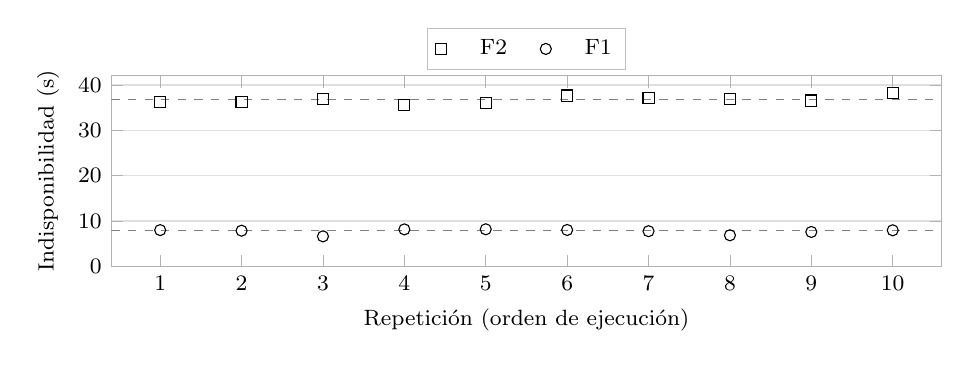
\begin{tikzpicture}
\begin{axis}[
  width=\columnwidth, height=4.0cm,
  xlabel={Repetición (orden de ejecución)},
  ylabel={Indisponibilidad (s)},
  label style={font=\footnotesize}, tick label style={font=\footnotesize},
  xmin=0.4, xmax=10.6, xtick={1,...,10},
  ymin=0, ymax=42, ytick={0,10,20,30,40},
  ymajorgrids=true, grid style={gray!25},
  axis line style={gray!60}, tick style={gray!60},
  legend style={font=\footnotesize, draw=gray!50, at={(0.5,1.03)},
                anchor=south, legend columns=2, column sep=1em},
]
\addplot[only marks,mark=square,mark size=2pt,draw=black] coordinates {(1,36.19) (2,36.21) (3,36.92) (4,35.51) (5,36.05) (6,37.66) (7,37.10) (8,36.95) (9,36.57) (10,38.32)};
\addlegendentry{F2}
\addplot[only marks,mark=o,mark size=2pt,draw=black] coordinates {(1,7.99) (2,7.86) (3,6.61) (4,8.15) (5,8.17) (6,8.02) (7,7.75) (8,6.85) (9,7.58) (10,7.95)};
\addlegendentry{F1}
\addplot[dashed,gray,domain=0.4:10.6,forget plot] {36.745};
\addplot[dashed,gray,domain=0.4:10.6,forget plot] {7.905};
\end{axis}
\end{tikzpicture}
\caption{Las diez repeticiones de cada escenario, en su orden de ejecución; las líneas
discontinuas marcan las medianas (7,905 y 36,745~s). Los lotes no se solapan. Las dos magnitudes no
son RTO comparables: la de F1 es un tiempo de recuperación por promoción de réplica, y la de F2,
el tiempo que se infiere que tarda el operador en deshacer la alteración que introdujo el inyector
(\refsec{sec:rtorpo}). En F2 se aprecia la deriva ascendente que recoge el coeficiente de
Spearman. Fuente: \texttt{data/f1\_rto\_cnpg.csv} y
\texttt{data/f2\_podfailure\_\allowbreak cnpg.csv} del paquete depositado.}
\label{fig:timeline}
\end{figure}

Los tres escenarios se articulan en torno a una misma variable, aunque no la que se anticipó. En F1 la eliminación del pod deja al plano de control sin primario; el operador registra el evento «\textit{Current primary isn't healthy, initiating a failover}» y promueve una réplica en $\approx 7{,}9$~s: es el único de los tres en que hubo una decisión de \textit{failover} que tomar. En F2 y F3 no hubo promoción porque no hubo fallo visible que la motivara —en F2 porque el inyector planteó una deriva de especificación en lugar de una indisponibilidad; en F3 porque el aislamiento fue parcial—. La variable que gobierna lo observado no es, entonces, el fallo nominal que el experimento pretende inducir, sino el estado en que el plano de control ve al primario; y ese estado lo fija tanto el fallo como el mecanismo de inyección empleado. De los cuatro escenarios diseñados, solo F1 produjo el fallo que decía producir: F4 ni siquiera llegó a ejecutarse (\refsec{sec:io}).

\subsection{Sensibilidad a la latencia de E/S}\label{sec:io}
El escenario F4 (sensibilidad del RTO a la latencia de E/S vía IOChaos) resultó no ejecutable sobre CNPG: el inyector de E/S de Chaos Mesh basado en FUSE (\texttt{toda}) falló al montar el sistema de archivos con \texttt{Read-only file system} porque CNPG endurece sus pods con \texttt{readOnlyRootFilesystem: true}, mientras que \texttt{toda} requiere una raíz escribible. No fue un error de configuración (el \textit{dry-run} de selectores y el recurso PodIOChaos eran correctos), sino una incompatibilidad entre ese inyector y el endurecimiento del operador —no una propiedad general de Chaos Mesh—. La medición cuantitativa se asigna a la Fase~2 por una vía que no dependa de FUSE (p.\,ej., \texttt{io.max} a nivel de \textit{cgroup}); el detalle completo está en el material suplementario.

\subsection{Contraste entre el comportamiento anticipado y el observado}\label{sec:contraste}
Se anticipaba, por el comportamiento documentado (Tabla~S2), que el fallo del pod primario dispara la promoción; F1 lo confirmó. Las otras dos expectativas —que la indisponibilidad sostenida promovería, y que una partición obligaría al sistema a elegir entre consistencia y disponibilidad— no llegaron a ponerse a prueba, porque ninguno de los dos escenarios construyó la condición que suponía (\refsec{sec:rtorpo}). no se refutaron, quedaron sin examinar.

La versión anterior proponía una regularidad: que la promoción estuviera condicionada a que el plano de control observase la pérdida de identidad del pod primario. Se retira. La evidencia disponible la contradice por dos vías independientes. Ante un fallo de nodo el objeto Pod no desaparece  (permanece en \textit{Terminating}) y, aun así, CNPG promueve. Y en el experimento de aislamiento completo ya citado hubo promoción con el pod del primario intacto y corriendo \citep{sivko2026}. El disparador documentado es más simple y da cuenta de los tres escenarios: el operador promueve cuando detecta la instancia primaria como no sana, sujeto a \texttt{failoverDelay}. En F1 la detectó; en F2 y F3 no llegó a haber nada que detectar.

El bloqueo de F4 apunta a una cuestión del mismo orden: la \textit{inyectabilidad} de un fallo depende del endurecimiento del operador. En conjunto, las cuatro observaciones apuntan a un problema conocido: la representatividad del fallo inyectado, sistematizada hace tiempo para la inyección de fallos de software \citep{natella2016}. Lo que este piloto añade es su forma específica ante un reconciliador declarativo: un inyector que muta la especificación del recurso no inyecta un fallo, sino una deriva del estado deseado, y el bucle de reconciliación la absorbe como cualquier otra. La semántica del inyector queda transformada por el sistema que pretende perturbar, de modo que acreditar que produce el fallo que nombra es condición previa a cualquier cifra de resiliencia. Las herramientas de prueba automática de controladores atacan el problema complementario, la corrección del operador ante secuencias de estados \citep{sun2022,gu2023}.


\section{Discusión}\label{sec:disc}
El piloto deja una lección que no se buscaba: el camino de un fallo hasta el motor de base de datos atraviesa capas que pueden impedir que llegue a plantearse como tal. En F2 el bucle de reconciliación del operador deshizo la perturbación antes de evaluar promoción alguna; en F3 la política de red nunca llegó a aislar al primario. La observación alcanza al operador y a la pila de red: la capa de almacenamiento gestionada mediante CSI no se ejercitó en este piloto \citep{avizienis2004}.

El alcance es una fase piloto acotada por el entorno productivo (\refsec{sec:metodo}). Cuatro limitaciones, por orden de peso. La primera, y la que más condiciona la lectura, es la \textit{fidelidad de la inyección}: F2 no reprodujo una indisponibilidad genuina y F3 no logró aislar al primario, por lo que ninguno de los dos sostiene conclusión alguna sobre la lógica de promoción del operador; la única medición de \textit{failover} que se sostiene es la de F1. La segunda: el fallo de nodo no se reprodujo —las tres instancias residían en un único nodo elegible—, por lo que el \textit{failover} medido es intranodo y el RPO nulo de F1 debe leerse como acotado por la ausencia de enlace de red internodo. La tercera: un solo operador y una sola categoría de almacenamiento, con el contraste entre operadores sostenido analíticamente (Tabla~S2) y no medido. La cuarta: F4 no fue ejecutable (\refsec{sec:io}). El valor del piloto no está, pues, en cuántos comportamientos caracteriza, sino en haber medido uno con precisión y haber identificado por qué los otros tres no eran medibles con el instrumental empleado.

Lo que este piloto no pudo resolver queda asignado a una Fase~2 ya diseñada, que se ejecutará en un clúster multinodo dedicado y fuera de producción, en el marco del Trabajo de Especialización en Desarrollo de Software de la FaCyT-UC. Su requisito previo es un protocolo de validación del inyector: cada escenario deberá acreditar, mediante los eventos del operador y el estado del pod ante el plano de control, que indujo el fallo que nombra antes de que su medición se dé por válida. Sobre esa base se abordan seis cuestiones —repetición de F2 sin tocar la especificación del pod, aislamiento completo en F3, fallo de nodo con antiafinidad obligatoria, F4 por \textit{cgroups}, instrumentación del retardo de replicación y comparación empírica entre operadores y clases de almacenamiento—, cuyo diseño detalla el material suplementario.

\section{Conclusiones}\label{sec:concl}
Este trabajo midió el coste del \textit{failover} de CloudNativePG en un clúster productivo, con inyección controlada de fallos y un verificador que registra, a nivel de \textit{commit}, qué escrituras confirmadas sobreviven. Ante la eliminación del pod primario promovió una réplica en las diez repeticiones, con un RTO mediano de 7,9~s y sin pérdida detectada: la tabla de verdad resultó contigua a lo largo de 613\,253 identificadores. Es una cifra de producción, con las restricciones que se declaran en la \refsec{sec:disc}.

El resultado de mayor alcance es metodológico y no estaba previsto: de los cuatro escenarios diseñados, solo uno reprodujo el fallo que nominalmente modela. El \textit{pod-failure} de Chaos Mesh altera la especificación del pod, y todo indica que un operador declarativo la trata como cualquier otra deriva del estado deseado (la comprobación directa queda para la Fase~2). La \textit{NetworkPolicy} no aisló al primario del plano de control, con lo cual la ausencia de promoción no expresó preferencia por la consistencia sino falta de detección: en un experimento independiente con aislamiento completo y configuración por defecto, CloudNativePG promovió y se perdieron escrituras confirmadas \citep{sivko2026}. Y el inyector de E/S resultó incompatible con el endurecimiento del propio operador. De ahí la conclusión que este trabajo defiende con más firmeza: en operadores declarativos el mecanismo de inyección no es un detalle de implementación sino parte de lo que se mide, y acreditar que produce el fallo que nombra debe preceder a cualquier cifra de resiliencia.

Se retira, por último, la regularidad que la versión anterior proponía —que la promoción dependiera de observar la desaparición del pod primario—: la contradicen la mecánica del desalojo por fallo de nodo y el experimento de \citet{sivko2026}. El disparador documentado, detectar una instancia no sana, basta para lo observado. El vocabulario $S=(O,K,M,D)$ se ofrece con el mismo carácter: andamiaje para organizar la observación por capas, no un modelo predictivo. Con el paquete de ejecución depositado, lo que este artículo entrega es una medición defendible, un diagnóstico de por qué las otras tres no lo son y un diseño corregido para obtenerlas.
